\documentclass{article}

% if you need to pass options to natbib, use, e.g.:
% \PassOptionsToPackage{numbers, compress}{natbib}
% before loading nips_2016
%
% to avoid loading the natbib package, add option nonatbib:
% \usepackage[nonatbib]{nips_2016}

\usepackage{nips_2016}

% to compile a camera-ready version, add the [final] option, e.g.:
% \usepackage[final]{nips_2016}

\usepackage[utf8]{inputenc} % allow utf-8 input
\usepackage[T1]{fontenc}    % use 8-bit T1 fonts
\usepackage{hyperref}       % hyperlinks
\usepackage{url}            % simple URL typesetting
\usepackage{booktabs}       % professional-quality tables
\usepackage{amsfonts}       % blackboard math symbols
\usepackage{nicefrac}       % compact symbols for 1/2, etc.
\usepackage{microtype}      % microtypography
\usepackage{graphicx}

\graphicspath{ {images/} }
\usepackage{xcolor}
\newcommand\todo[1]{\textcolor{red}{#1}}


\title{Forward Thinking}

% The \author macro works with any number of authors. There are two
% commands used to separate the names and addresses of multiple
% authors: \And and \AND.
%
% Using \And between authors leaves it to LaTeX to determine where to
% break the lines. Using \AND forces a line break at that point. So,
% if LaTeX puts 3 of 4 authors names on the first line, and the last
% on the second line, try using \AND instead of \And before the third
% author name.

\author{
  Math People\thanks{Use footnote for providing further
    information about author (webpage, alternative
    address)---\emph{not} for acknowledging funding agencies.} \\
  Department of Mathematics\\
  Brigham Young University\\
  Provo, UT 84602\\
  \texttt{seanwade@byu.edu} \\
  %% examples of more authors
  %% \And
  %% Coauthor \\
  %% Affiliation \\
  %% Address \\
  %% \texttt{email} \\
  %% \AND
  %% Coauthor \\
  %% Affiliation \\
  %% Address \\
  %% \texttt{email} \\
  %% \And
  %% Coauthor \\
  %% Affiliation \\
  %% Address \\
  %% \texttt{email} \\
  %% \And
  %% Coauthor \\
  %% Affiliation \\
  %% Address \\
  %% \texttt{email} \\
}

\begin{document}
% \nipsfinalcopy is no longer used

\maketitle

\begin{abstract}
  We propose a new method for the layer-wise dynamic training of neural networks without backpropegation. This method begins with a low level classifier and dynamically adds layers until learning does not improve. Removing back propegation also removes the need for predetermined computational graphs. This frees the network to grow the archetecture as it needs. The result is quicker training time as well as higher accuracy.
\end{abstract}

\section{The Method}

This is how I implemented the architectures. These methods draw inspiration from the layerwise training of Deep Belief Networks as well as the graph augmentation of the guy tanner said.

\subsection{Forward Thinking}

The base of forward thinking is feature engineering while training the network. In its most simple form this looks like using the loss function to have a low level learner try to classify by using one hidden layer. This layer can be interpreted as the learned features. When ready to increase learning ability the data is training data is transformed using these features. The next iteration of the algorithm takes the old features and the new features to attempt to learn the problem. A weakness to this method is there is limited transfer of learned knowledge when attempting to learn the next layer. This knowledge only lies in the form of the new features. This can be seen at training time with sharp drops in accuracy at new layers.

\begin{center}
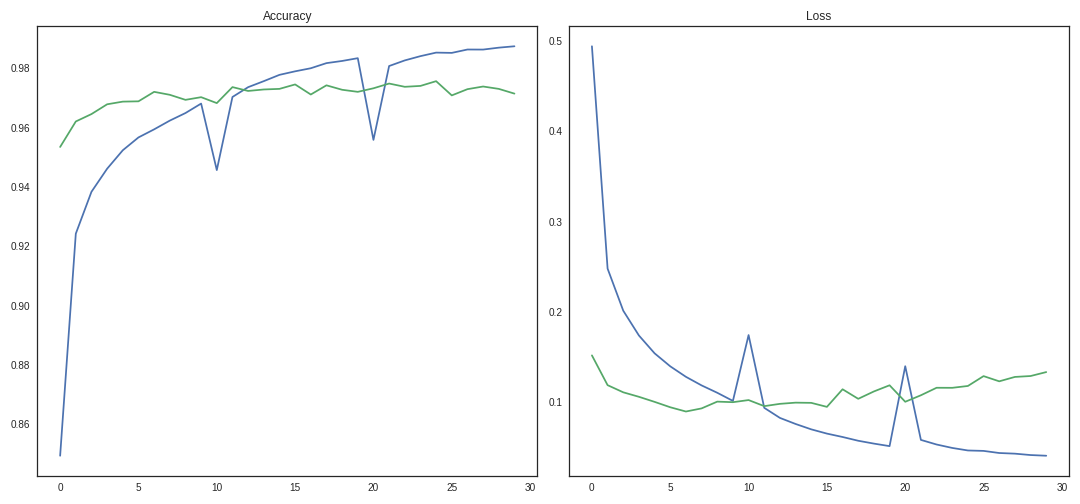
\includegraphics[scale=.25]{acc-loss-forward-thinking}
\end{center}

\subsection{Pass-Forward Thinking}

To overcome the obstacles in the aforementioned section, we introduce information preserving pass-forward thinking. Similar to work by that one guy tanner cited, we intelligently add layers to the model, such that knowledge caries over and there is no drop in accuracy. In the case of standard DNN's this has an elegant representation.

\begin{center}
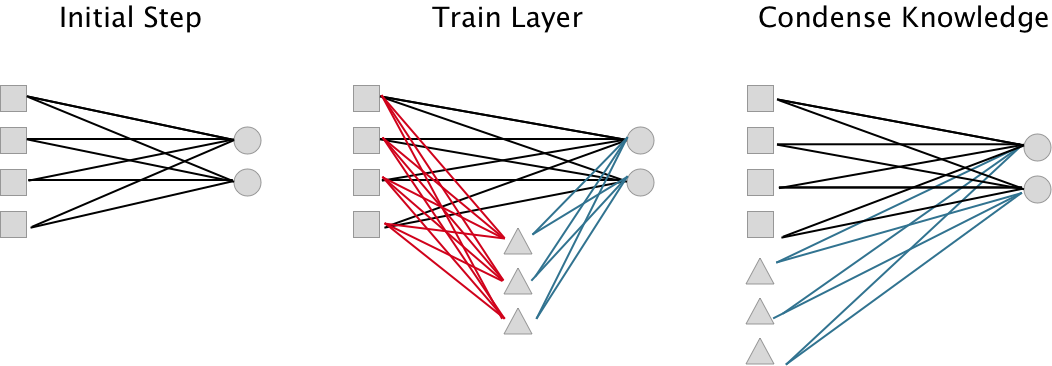
\includegraphics[scale=.30]{flow-diagram}
\end{center}

The matrix represented by the black connections can be described as the knowledge matrix learned from previous layers. The red connections are the transformation matrix, the connections that generate the new features. Finally, the blue connections are the new knowledge. With our new features, this information connects directly to the output. In the final stage we flatten both the old and new knowledge to get a single representation.

We note that with this method of training we have two options: freeze old knowledge or continue to train it. It seems to be that freezing outperforms. I speculate this is because it serves as a form of regularization and allows the network to not have to focus on tweaking everything at once.

\subsection{Push-Forward Thinking}

Push-Forward Thinking is method for growing neural networks deeper to improve learning. Our method allows doing so without a loss in accuracy (hopefully). This dynamic topology overcomes the weakness of standard neural networks by not having to predetermine the depth. It also eliminates the need for back propagation.

\subsection{Thoughts}

Each of these implementations offer different spins on the idea of forward thinking by pushing the data through while training. Pass-forward allows any number of hidden nodes to be added in the subseqwuent layers. This overcomes the weaknesses of cascase correlation learning, which only adds a single neuron? Whe we did this on MNIST it only was ably to get 96.34\% accuracy since the added learners were too weak to gain any meaningful insite on their own. Push through has the limitation of having the same amount of hidden neurons in each layer. 

\begin{center}
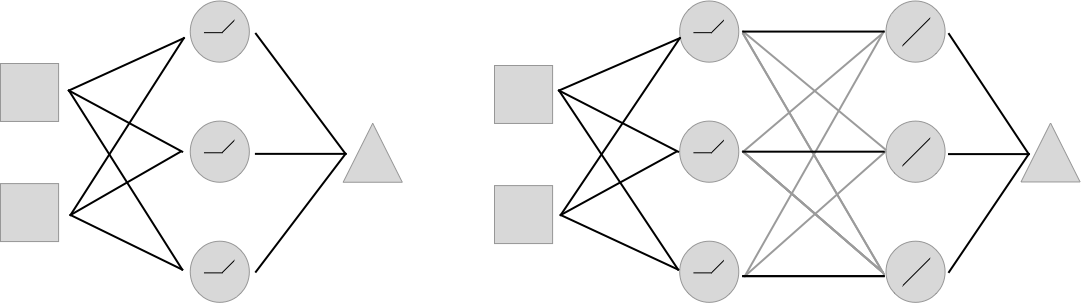
\includegraphics[scale=.22]{push-forward}
\end{center}


\section{Observations}

\subsection{Freezing Features}

Once the network has plateued, the layers are then frozen and more layers are added to increase the compacity to  learn. This method of training comes with several benifits as wll as tradeoffs. The first benifit is increased learning speeds. A typical neural network must learn all the weights at once. By starting with fewer weights, these can be learned faster as is seen in the following graphic.


\begin{center}
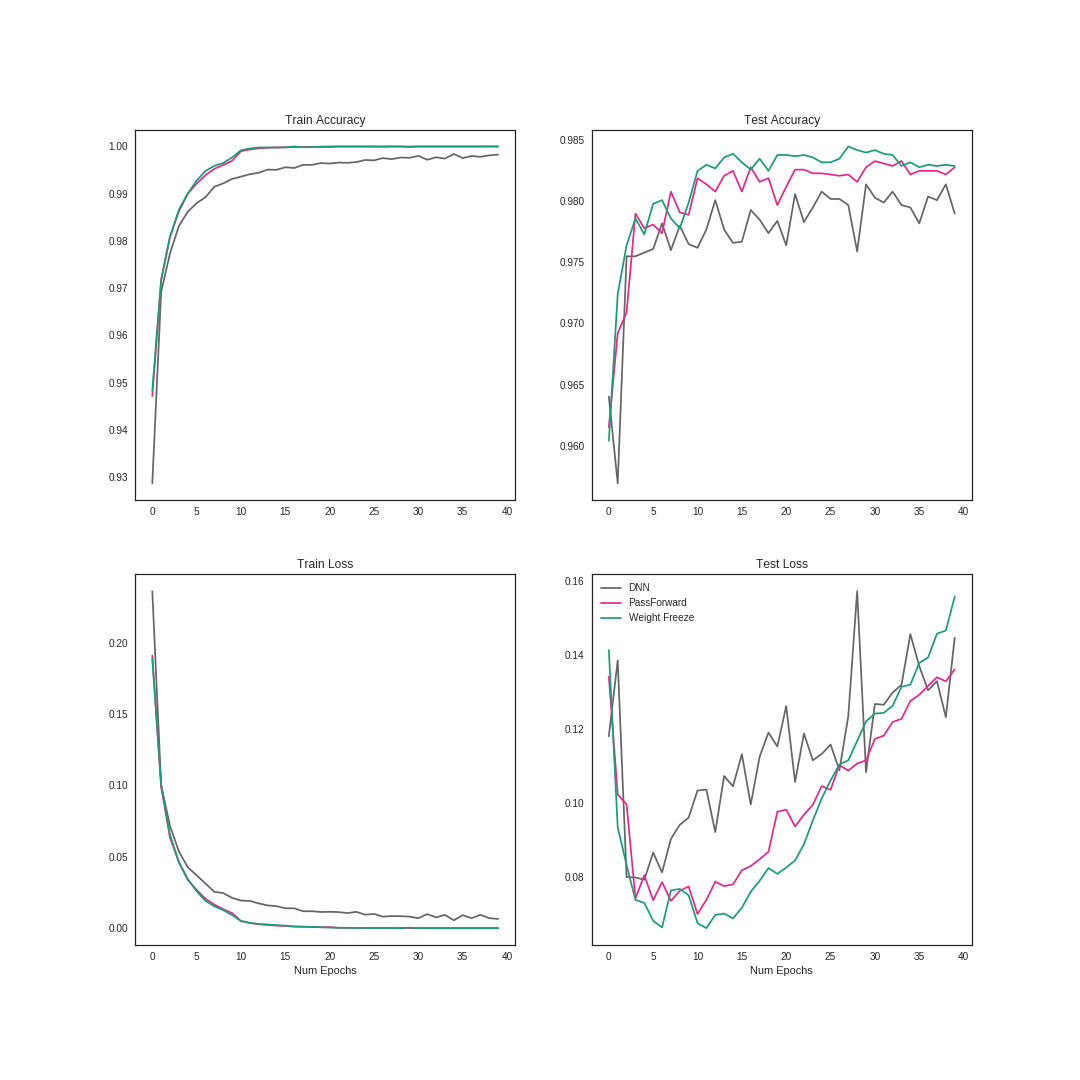
\includegraphics[scale=.32]{comparison}
\end{center}

Another benifit of freezing features is that it serves as a natural form of regularization. Once general concepts are learned, layers are frozen to prevent overfitting by hyper tuning the parameters. Now thats a win.

\subsection{Greedy Algorithm}

A weakness of elimenating backprop is that forward thinking is a gready algorithm. If the data is transformed with each layer then data is lost and it learnes the best it can even though that may not be optimal. We saw this when doing the pure push data through approach.

We were able to combat this by using an approach similar to res-nets. That is that we would still input the primary features into subsequent layers. This improved accuracy and allowed the network to recover from greedy learning later down the line in training.

\subsection{Other Random}

\begin{itemize}
\item Focus on building whole network from scratch, dynamic
\item No backprop
\item Forward Thinking learns quicker than backprop, the accuracy only catches us when they both run a long time.

\end{itemize}


\section{Results}

\subsection{Regularization}

In working with the MNIST dataset we implemented many different types of regularization. These included l1, l2, as well as dropout. Both the regular DNN and Forward THining implementations would get comparable results to before. With this being such a simple problem there were no noteworthy increases in accuracy in any of the methods. But it is important to note that these results were the same with a plain DNN structure. It is very likely that the benifits of regularization will extend in the same places they do with DNNs. \todo{If we can find a good dataset to show this with that would be nice.}


\begin{table}[h]
  \caption{MNIST without augmentation}
  \label{mnist-table}
  \centering
  \begin{tabular}{lll}
    \toprule                
    Name     & Accuracy & Training Time (seconds) \\
    \midrule
    DNN &     97.9\%   & 265.93 \\
    Forward Thinking  & 97.9\% & 174.81  \\
    Pass-Forward Thinking  & 98.28\%  & 239.07 \\
    Pass-Forward Thinking  (weight freeze)& 98.29\% & 231.42 \\
    \bottomrule
  \end{tabular}
\end{table}

\begin{table}[h]
  \caption{MNIST with augmentation}
  \label{mnist-table}
  \centering
  \begin{tabular}{lll}
    \toprule                
    Name     & Accuracy & Training Time (seconds) \\
    \midrule
    DNN &     98.78\%   & slowest \\
    Forward Thinking  & 98.80\% &  2 fastest\\
    Pass-Forward Thinking  & 98.87\%  & 3 fastest\\
    Pass-Forward Thinking  (weight freeze) & 98.85\% & 1 fastest \\
    \bottomrule
  \end{tabular}
\end{table}

\todo{Make the time and accuracy relative}

\begin{itemize}
\item The weight freezing is significantly faster than not for the augmented data. 
\item the abovce results are a 3 layer deep network, 150, 100, 50. Adding a 4th layer had no improvment in accuracy
\item My code is on the github if there are other things anybody wants to try
\end{itemize}

\section{Future Work}

\begin{itemize}
\item How to determine width of adding layer in pass-forward
\item look at learned features at every layer
\item Use similar method for other machine learning models by stacking them and passing through the data
\item CNN's
\item Optimization methods build specifically with this in mind
\item When to best know when to add a layer, is it just accuracy dosnt change for 5 epcohs or is there something better?
\end{itemize}

\section*{References}


\end{document}
